\documentclass[11pt,a4paper]{article}
\usepackage[T1]{fontenc}
\usepackage{lmodern,amsmath,amssymb,amsthm,mathtools,booktabs,graphicx,microtype}
\usepackage[margin=25mm]{geometry}
\usepackage{xcolor}
\usepackage[colorlinks=true,linkcolor=blue!45!black,urlcolor=blue!50!black]{hyperref}
\usepackage{fancyhdr,needspace}
\pagestyle{fancy}\fancyhf{}\lhead{Causal recovery from a weak quantum stream}\rhead{5 November 2026}\cfoot{\thepage}
\setlength{\headheight}{14pt}
\setlength{\parindent}{0pt}\setlength{\parskip}{6pt}
\newtheorem{theorem}{Theorem}
\newtheorem{corollary}{Corollary}
\newcommand{\id}{\operatorname{id}}
\newcommand{\Tr}{\operatorname{Tr}}
\newcommand{\SWAP}{\operatorname{SWAP}}
\newcommand{\dd}{d_\diamond}
\newcommand{\R}{\mathcal R}
\newcommand{\norm}[1]{\left\lVert#1\right\rVert}
\title{\vspace{-1em}Causal recovery from a homogeneous\\weak quantum stream\\[.45em]\large Quantitative memory lower bounds, exact carrier-loss bounds,\\and the unresolved scaling question}
\author{Research construction and reproducibility note}
\date{5 November 2026}
\begin{document}
\maketitle
\begin{abstract}
The fixed endpoint is a causal decoder for an arbitrary qubit emitted through a homogeneous weak partial-SWAP stream, attaining the quartic collision scale with genuinely sublinear quantum storage and near-linear processing, or a matching general obstruction. This investigation does not resolve that endpoint. A crossing and interpolation argument establishes an explicit positive singular gap for every finite prefix. Combined with a strengthened general instrument converse, this forces quantum memory $\Omega(\log(1/\epsilon)/\log\log(1/\epsilon))$ at each fixed nonzero angle, or $\Omega_\theta(N/\log N)$ at the benchmark count. It rules out every fixed polynomial saving in storage in that regime, while leaving a logarithmic gap to the known reader. Exact one- and two-qubit error floors and a carrier-erasure law are also derived. The joint weak-angle limit and the full memory/processing tradeoff remain unresolved.
\end{abstract}

\section{The endpoint remains fixed}
One source qubit $S$, initially in an arbitrary state possibly entangled with an inaccessible reference, meets fresh independent carriers $E_j$ in $\tau=I/2$. Each encounter uses the known gate
\[
 U_j=cI+is\SWAP_{S,E_j},\qquad c=\cos\theta,\quad s=\sin\theta,\qquad 0<\theta<\pi/2.
\]
The receiver sees each emitted carrier once in chronological order. The final source is discarded. The receiver may use initialized workspace, arbitrary instruments, classical records, feedback and buffers. All coherent registers crossing a time cut count as quantum memory. Bath purifiers, preparation keys and a return link to the source are unavailable.

Write $\mathcal C_N$ for the acquired channel and use half-diamond error
\[
 \dd(\mathcal D\mathcal C_N,\id)=\tfrac12\norm{\mathcal D\mathcal C_N-\id}_\diamond.
\]
The full question asks for a physical causal operation with this error at most $\epsilon$, collision count $N=\Theta(\theta^{-4}\log(1/\epsilon))$, genuinely sublinear retained quantum memory, and near-linear processing, with the resource dependence exposed jointly. A failure of a particular receiver does not answer that question. Nor does a compressed description of an operator establish a physically implementable quantum memory.

Partial-SWAP homogenization itself is established research [1]. General transpose/Petz recovery and its near-optimality are also established machinery [2,3]. The exact source-specific all-output benchmark used here is the earlier Astra return [A1]. The recent general memory converse is [A2]. These are reused, rather than claimed as discoveries in this run.

\section{The accepted all-output benchmark}
Let $b=s^4$ and $r=1-b$. Retain all $N$ outputs, prepare a separate mixed dummy qubit, and apply the inverse collisions to the dummy in reverse chronological order. This is an output-only operation. The actual source is not supplied. Its exact recovered channel is
\begin{equation}
 \mathcal D_N\mathcal C_N=(1-r^N)\id+r^N\R_{I/2},\qquad
 \dd(\mathcal D_N\mathcal C_N,\id)=\tfrac34r^N.
 \label{eq:benchmark}
\end{equation}
Every unrestricted decoder of the full output obeys [A1]
\begin{equation}
 \epsilon_{\rm opt}\ge\tfrac34\bigl(1-\sqrt{1-r^N}\bigr).
\end{equation}
Thus the explicit operation is within a factor two in error of this lower bound. A sufficient count is
\begin{equation}
 N_{\rm all}=\left\lceil\frac{\log(3/(4\epsilon))}{-\log(1-\sin^4\theta)}\right\rceil.
\end{equation}
At $\theta=0.1$ and $\epsilon=0.01$, it requires $43\,462$ encounters; the unrestricted converse requires at least $36\,552$. Source marginal forgetting instead has visibility $c^{2N}$ and therefore a quadratic weak-angle clock. Forgetting and accessible recovery are distinct operations.

The abstract decoder uses $N$ stored carrier qubits, one dummy, and $N$ addressed inverse two-qubit gates. Physical routing, service backlog, protection and calibration must also be counted. Linear addressed gate count is not a geometry-independent linear-time implementation.

\section{A strengthened converse for general causal receivers}
The recent Astra note [A2] supplies a general spectral-profile reduction. The following construction retains that reduction and improves its finite-error coefficient using established sharp recovery machinery. At prefix length $L$, let $D=2^L$ and define the bistochastic bath channel
\[
 T_L(K)=\tfrac12\Tr_S\!\left[U^{(L)}(I_S\otimes K)U^{(L)\dagger}\right],
 \qquad H_L=I-T_LT_L^*.
\]
Write its eigenvalues in increasing order as $\lambda_0,\ldots,\lambda_{D^2-1}$. For a converse, grant the receiver the actual source at this cut. It can simulate the future from there, so this only helps recovery.

The previous coefficient in [A2] was $3\epsilon(1-\epsilon)$. We obtain the following strengthened witness for $0\le\epsilon\le1/2$.

\begin{theorem}[Refined-instrument spectral witness]
Any successful receiver whose quantum capacity in every classical branch at the cut is at most $m$ induces a bistochastic Choi witness $Z$ with
\[
 \Tr Z=1,\qquad 0\le Z\le(m/D)I,\qquad
 \Tr(H_LZ)\le e_\epsilon:=2\epsilon-\tfrac43\epsilon^2.
\]
This includes arbitrary initialized workspace, instruments and classical histories. If $D/m$ is an integer, it implies
\begin{equation}
 \frac{m}{D}\sum_{j=0}^{D/m-1}\lambda_j\le e_\epsilon.
 \label{eq:profile}
\end{equation}
For every $t>0$ there is also the heat-trace bound
\[
 m\ge\frac{D\exp[-t e_\epsilon]}{\Tr\exp(-tH_L)}.
\]
\end{theorem}

\begin{proof}
Refine each branch of the prefix instrument into its individual Kraus outcomes. Revealing this refinement only helps the receiver. Each Kraus map $K_x:\mathbb C^D\to M_x$ has rank at most $m$. Set
\[
 A_x=(K_x^\dagger K_x)^{1/2},\qquad
 \sum_xA_x^2=I,\qquad
 \mathcal L(X)=\sum_xA_xXA_x.
\]
The polar isometry in $K_x$ is undone by the branch Petz map. Since the logical maximally mixed input is mapped by the reversible prefix encoder to $I_S/2\otimes I/D$, the logical-channel Petz composition is precisely: encode, apply $\id_S\otimes\mathcal L$, undo the prefix unitary and trace the bath. A logical Pauli twirl therefore gives its entanglement fidelity as
\[
 F_{\rm P}=\frac1D\sum_x\norm{T_L^*(A_x)}_2^2.
\]
Here the norm is the ordinary, unnormalized Hilbert--Schmidt norm. With ordinary matrix vectorization, define
\[
 Z=\frac1D\sum_x|A_x\rangle\!\rangle\langle\!\langle A_x|.
\]
Then $\Tr Z=1$, both marginals are $I/D$, and exactly
\[
 \Tr(H_LZ)=1-F_{\rm P}.
\]
For an arbitrary matrix $B$, Cauchy--Schwarz on the support of $A_x$ gives
\[
 |\Tr(B^\dagger A_x)|^2\le m\Tr(A_x^2BB^\dagger).
\]
Summing proves $Z\le(m/D)I$.

The sharp qubit Petz bound [2, Eq. (13)] is
\[
 F_{\rm P}\ge F^2+\frac{(1-F)^2}{3}
\]
for the entanglement fidelity $F$ of any recovery. Half-diamond error at most $\epsilon$ gives $F\ge1-\epsilon$. The right side increases for $F\ge1/4$, so $1-F_{\rm P}\le2\epsilon-4\epsilon^2/3$ for $\epsilon\le3/4$.

For completeness, this recovery inequality also follows directly by applying the order-two sandwiched R\'enyi data-processing inequality to the two-outcome Bell test after recovery. Its success probability on the normalized channel Choi state is $F$, and on the product of the uniform reference and the channel output average is $1/4$. The resulting binary expression is $4F^2+(4/3)(1-F)^2$, while the initial expression is $4F_{\rm P}$.

The density cap minimizes energy by filling the smallest eigenvalues first, proving \eqref{eq:profile}. Jensen's inequality and the same cap give $e^{-t e_\epsilon}\le\Tr(Ze^{-tH_L})\le(m/D)\Tr(e^{-tH_L})$.
\end{proof}

For noninteger $D/m$, write $a=m/D$ and $k=\lfloor1/a\rfloor$. The exact profile condition is $a\sum_{j=0}^{k-1}\lambda_j+(1-ka)\lambda_k\le e_\epsilon$. If $n_L(u)$ counts eigenvalues below $u>0$, then $m\ge D[1-e_\epsilon/u]_+/n_L(u)$. Grouping the refined Kraus terms by the original branch gives, for variable capacity $m_y$,
\[
 \Pr(m_y>m)\ge[1-e_\epsilon/u-m n_L(u)/D]_+.
\]
The probability is the branch law under the tracial bath marginal. Summing tail bounds gives expected occupancy bounds as in [A2]. These conditions remain necessary, not sufficient for a compression channel. The new coefficient is strictly smaller than the old one for $0<\epsilon<3/5$, including the entire stated range $\epsilon\le1/2$.

\subsection{An explicit gap at every prefix length}
The central additional step is a quantitative bound on the singular defect, with no extrapolation from small matrices.
\begin{theorem}[All-prefix crossing bound]
For $u=\cot\theta>0$ and $n\ge1$, define
\[
 B_n=\frac{u^2+4n^2}{u},\qquad K_n=\frac{B_n^n[(u+2n)^n+1]}{n!},\qquad
 g_n=\frac6{n(n+1)(2n+1)K_n^2}.
\]
Then
\begin{equation}
 \gamma_n:=1-\norm{T_n|_{\mathbf1^\perp}}_{2\to2}^2\ge g_n>0.\label{eq:allgap}
\end{equation}
The identity is the only zero mode of $I-T_nT_n^*$. At fixed $\theta$, $\log g_n=-4n\log n+O_\theta(n)$.
\end{theorem}
\begin{proof}
Use normalized Hilbert--Schmidt norms unless an operator norm is specified. Define
\[
 M_n(z)=(zI+iP_{S,n})\cdots(zI+iP_{S,1}),\qquad U^{(n)}=(u^2+1)^{-n/2}M_n(u).
\]
For $\mathcal C(A)=(\sigma_y\otimes I)A^{t_S}(\sigma_y\otimes I)$, the local identity $\mathcal C(P)=I-P$ implies
\begin{equation}
 \mathcal C[M_n(z-i)]=(z^2+1)^nM_n(z)^{-1}.\label{eq:cross}
\end{equation}
The bath entries in distinct local factors commute, justifying their reversed order under source transpose. No general multiplicativity of partial transpose is assumed. The map $\mathcal C$ preserves Hilbert--Schmidt norm.

Take a traceless bath operator $X$ of norm one, set $Y=T_n(X)$, and write $\widehat X=I_S\otimes X$, $\widehat Y=I_S\otimes Y$. Source conditional expectation is an orthogonal projection, so
\[
 \delta^2:=\norm{U^{(n)}\widehat XU^{(n)\dagger}-\widehat Y}^2=1-\norm{T_n(X)}^2.
\]
For $E(z)=\widehat YM_n(z)-M_n(z)\widehat X$, one has $\norm{E(u)}=(u^2+1)^{n/2}\delta$. If $\widetilde E$ interchanges $X,Y$, crossing gives
\[
 \widetilde E(z-i)=-(z^2+1)^n\mathcal C[M_n(z)^{-1}E(z)M_n(z)^{-1}].
\]
Thus the pair alternates under each shift, returning after two shifts. This matters because norm preservation initially gives an intertwiner, not a commutant.

At $z=u-ik$, each local inverse has operator norm at most $[u^2+(k-1)^2]^{-1/2}$. The norm multiplier per shift is at most
\[
 \left[\frac{u^2+(k+1)^2}{u^2+(k-1)^2}\right]^{n/2}.
\]
These factors telescope. At the $n+1$ even-shift points, $\norm{E(u-2ij)}\le B_n^n\delta$, $j=0,\ldots,n$.

Interpolate the degree-$n$ polynomial $E$. The sum of absolute leading-coefficient weights is $\sum_{j=0}^n[2^nj!(n-j)!]^{-1}=1/n!$. The leading coefficient is $\widehat Y-\widehat X$; the interpolation weights at zero have numerators bounded by $(u+2n)^n$. Hence
\[
 \norm{Y-X}\le B_n^n\delta/n!,\qquad
 \norm{E(0)}\le B_n^n(u+2n)^n\delta/n!.
\]
Since $M_n(0)$ is a unit phase times the cyclic permutation $C$ of all $n+1$ sites, $\norm{[\widehat X,C]}\le K_n\delta$.

Let $P_j$ be the normalized partial-trace conditional expectation making site $j$ identity, where $j=0$ is the source. These projections commute. Since $P_0\widehat X=\widehat X$, cyclic rotation and telescoping give $\norm{(I-P_j)\widehat X}\le jK_n\delta$. Their joint projection is the scalar projection and vanishes on $\widehat X$. Therefore
\[
 1\le\sum_{j=1}^n\norm{(I-P_j)\widehat X}^2
 \le\frac{n(n+1)(2n+1)}6K_n^2\delta^2.
\]
This proves the bound. The two orientations $I-T_n^*T_n$ and $I-T_nT_n^*$ share the same singular defects. Stirling's formula gives the asymptotic exponent.
\end{proof}

\subsection{Consequence for arbitrary growing memory}
The witness has weight at most $m/2^n$ on the identity vector. Its energy and \eqref{eq:allgap} imply
\begin{equation}
 \frac m{2^n}\ge1-\frac{e_\epsilon}{g_n},\qquad
 q_n=\log_2m\ge n+\log_2(1-e_\epsilon/g_n),\label{eq:finiteq}
\end{equation}
when $e_\epsilon<g_n$. This bound is explicit jointly in $n,\theta,\epsilon$, but can be weak at moderate accuracy.

At fixed $\theta$, put $L_\epsilon=\log(1/\epsilon)$ and take
\[
 n=\left\lfloor\frac{(1-\eta)L_\epsilon}{4\log L_\epsilon}\right\rfloor,\qquad0<\eta<1.
\]
Then $g_n/\epsilon\to\infty$ and $q_n\ge n-o(1)$. Provided the stream reaches this cut,
\begin{equation}
 \liminf_{\epsilon\to0}\frac{q_{\rm peak}\log\log(1/\epsilon)}{\log(1/\epsilon)}\ge\frac14.\label{eq:asymemory}
\end{equation}
Logarithms here are natural; $q$ counts qubits. The branch-tail bounds give the same leading asymptotic for expected occupancy in the Bell-input experiment: use a threshold below $g_n$, where the low-energy mode count is one, then sum the memory tails.

At $N=\Theta_\theta(\log(1/\epsilon))$, including the quartic benchmark at fixed angle, this is $q_{\rm peak}=\Omega_\theta(N/\log N)$. It excludes $O(N^{1-\alpha})$ memory for every fixed $\alpha>0$ in that regime, with arbitrary classical memory and processing allowed. It still permits an $N/\log N$-type receiver. The angle dependence is not uniform: the explicit $g_n$ exposes it. No quartic memory lower bound as $\theta\to0$ at fixed error follows from this argument.

\subsection{General one- and two-qubit memory floors}
Let $\gamma_L$ be the minimum eigenvalue of $H_L$ on the traceless subspace, including any further zero modes if present. The witness has weight at most $m/D$ on the identity vector. Hence
\[
 e_\epsilon\ge\gamma_L(1-m/D).
\]
When $\gamma_L>0$, this yields
\begin{equation}
 \epsilon\ge\frac34\left[1-\sqrt{1-\frac43\gamma_L(1-m/D)}\right].
 \label{eq:gapfloor}
\end{equation}
At two carriers, the exact weak-angle gap is
\[
 \gamma_2=2\sin^4\theta-\sin^8\theta,
 \qquad \tan^4\theta\le\tfrac13.
\]
Thus every receiver with at most one persistent qubit after the second carrier has a lower-bound expansion $\theta^4/2+O(\theta^6)$, independent of the number of subsequent carriers.

At three carriers, exact symbolic perturbation gives
\begin{equation}
 \gamma_3=\frac{7-\sqrt{33}}2\theta^4+O(\theta^6).
\end{equation}
Consequently every receiver with at most two persistent qubits after the third carrier has the error floor
\begin{equation}
 \epsilon\ \ge\ \frac{7-\sqrt{33}}8\theta^4-C\theta^6
 \quad\text{for sufficiently small }\theta>0
 \label{eq:twoqubit}
\end{equation}
for some finite constant $C$. The positive leading coefficient is approximately $0.15693$. All classical histories and arbitrary subsequent operations are included.

An exact coefficient certificate is as follows. Set $t=\tan\theta$. The source-traceless leakage map has expansion $R(t)=tA+t^2B+O(t^3)$. Its first-order kernel is the five-dimensional SU(2)-scalar sector. Besides the identity, use
\[
 K_1=\boldsymbol\sigma_1\!\cdot\!\boldsymbol\sigma_2,\quad
 K_2=\boldsymbol\sigma_1\!\cdot\!\boldsymbol\sigma_3,\quad
 K_3=\boldsymbol\sigma_2\!\cdot\!\boldsymbol\sigma_3,\quad
 K_4=\sum_{abc}\epsilon_{abc}\sigma_{1a}\sigma_{2b}\sigma_{3c}.
\]
Their normalized Gram matrix is $G=\operatorname{diag}(3,3,3,6)$. Eliminating the first-order complement gives the effective metric
\[
 K^*B^*\bigl[I-A(A^*A)^+A^*\bigr]BK
 =\begin{pmatrix}6&3&-3&0\\3&18&3&0\\-3&3&6&0\\0&0&0&12\end{pmatrix}.
\]
Its eigenvalues relative to $G$ are $(7-\sqrt{33})/2$, $2$, $3$, and $(7+\sqrt{33})/2$. The other 59 traceless leakage modes start at positive order $\theta^2$. Analytic perturbation and angle-sign symmetry give the stated remainder. The accompanying exact-arithmetic script constructs the local Liouville maps and this matrix; it does not fit a numerical power law.

These floors exclude bounded one- and two-qubit solutions with arbitrarily small error at a fixed sufficiently weak angle. They do not exclude a receiver whose quantum memory grows sublinearly with $N$, or establish a large error at every practical tolerance.

The all-prefix bound proves \eqref{eq:asymemory}, but is not sharp enough to settle every sublinear memory scaling. Spectra of a different local random eSWAP process cannot be substituted without a proved comparison. Integrable transfer-matrix eigenvalues also do not directly give these singular values: the homogeneous transfer problem can have Jordan blocks [5].

A conditional observation isolates the remaining loss in this route. A bound $\gamma_L\ge a(\theta)e^{-b(\theta)L}$ would allow a cut $L$ proportional to $N$ and exclude a uniform $o(N)$ memory claim as $\epsilon\to0$ at fixed angle. Our proved bound has an additional $\log L$ in its exponent. No argument removing that factor is proved here. The padding identity in [A2] gives exponentially small \emph{upper} bounds on certain losses; it cannot be used as a lower bound.

\section{Exact erasure extension}
Fix an input-independent retained set $A\subseteq\{1,\ldots,N\}$. All other carriers are erased before receiver processing; the set is provided as a classical flag. Subsequent decoding on the retained outputs is unrestricted. Put $d=c^4$.

\begin{theorem}[Retained-carrier law]
Initialize $a_0=0$, $q_0=1$ and update chronologically by
\begin{align}
 j\in A:\quad &a_j=a_{j-1}+bq_{j-1},&q_j&=(1-b)q_{j-1},\label{eq:kept}\\
 j\notin A:\quad &a_j=a_{j-1},&q_j&=dq_{j-1}.\label{eq:lost}
\end{align}
There is a physical decoder $\mathcal D_A$ for which
\begin{equation}
 \mathcal D_A\mathcal C_A=a_N\id+(1-a_N)\R_{I/2},\qquad
 \dd(\mathcal D_A\mathcal C_A,\id)=\tfrac34(1-a_N).
 \label{eq:erasuredecoder}
\end{equation}
Every decoder of all retained outputs satisfies
\begin{equation}
 \epsilon_{\rm opt}(A)\ge\tfrac34(1-\sqrt{a_N}).\label{eq:erasurelower}
\end{equation}
\end{theorem}

\begin{proof}
Propagate any initial source Pauli through the collision circuit and immediately trace an erased carrier. This equals tracing it at the end, since it never returns. Use normalized Hilbert--Schmidt inner products, and split the signal into its source-identity part $P$ and source-traceless part $Q$. Let their squared norms be $a$ and $q$.

Old $P$ remains unchanged in the next collision. For any traceless source coefficient, partial SWAP sends its source-identity component to $s^2$ times the corresponding fresh-carrier Pauli. This export is orthogonal to old $P$ because the fresh Pauli is trace zero. Its squared norm is $s^4q$. Unitarity leaves $(1-s^4)q$ in the orthogonal $Q$ sector. This proves \eqref{eq:kept}, including arbitrary operator coefficients on older carriers. If the fresh carrier is erased, the source map is depolarizing with visibility $c^2$, so $Q$ has squared norm $c^4q$ and no new export survives. This proves \eqref{eq:lost}.

For $m=|A|$, write the retained-output channel as
\[
 \mathcal C_A\bigl((I+\boldsymbol u\cdot\boldsymbol\sigma)/2\bigr)
 =2^{-m}\bigl(I+\textstyle\sum_k u_kB_k\bigr).
\]
The preceding calculation and polarization give
\[
 2^{-m}\Tr(B_kB_l)=a_N\delta_{kl},\qquad \Tr B_k=0.
\]
The average output is exactly maximally mixed. Its Petz map is therefore the dimension-normalized adjoint $\mathcal D_A=2^{m-1}\mathcal C_A^*$. The Gram identity proves \eqref{eq:erasuredecoder}.

This adjoint is physical: start a mixed dummy, traverse the schedule backwards, apply $U^\dagger$ to each retained carrier, and at every erased position apply dummy depolarization of visibility $c^2$. A fresh mixed qubit, an inverse partial SWAP and discarding that qubit implement each replacement step.

Finally $\norm{\mathcal C_A(\sigma_k)}_1\le2\sqrt{a_N}$ by Hilbert--Schmidt Cauchy--Schwarz. A decoder contracts trace norm. Its entanglement fidelity with the identity is consequently at most $(1+3\sqrt{a_N})/4$. Testing its normalized Choi state with the Bell projector gives \eqref{eq:erasurelower}. The upper/lower error ratio is $1+\sqrt{a_N}\le2$ whenever the lower bound is nonzero.
\end{proof}

\subsection{Independent flagged loss}
Suppose each carrier is retained independently with probability $p=1-\ell$. Independence from the payload and the other erasures is essential. Define
\[
 f=p(1-b)+(1-p)d,\qquad
 \bar a_N=pb\frac{1-f^N}{1-f}.
\]
Averaging the exact recurrence gives this expression. The flagged branchwise Petz decoder has visibility $\bar a_N$ and error $\tfrac34(1-\bar a_N)$. Any decoder of the complete flagged output has error at least
\[
 \tfrac34\bigl(1-\sqrt{\bar a_N}\bigr),
\]
because $\mathbb E\sqrt{a_N}\le\sqrt{\mathbb E a_N}$. These are unconditional channel guarantees, including the loss flags.

As $N\to\infty$,
\begin{equation}
 \bar a_\infty=
 \frac{(1-\ell)\sin^4\theta}
 {(1-\ell)\sin^4\theta+\ell(1-\cos^4\theta)}.
 \label{eq:ainf}
\end{equation}
Acquisition contributes at fourth order, while losing a carrier attenuates the still-encoded signal at second order. In particular,
\begin{equation}
 \ell=\kappa\theta^2\quad\Longrightarrow\quad
 \bar a_\infty\longrightarrow\frac1{1+2\kappa}\qquad(\theta\to0).
\end{equation}
If $\ell/\theta^2\to\infty$, the optimal error tends to $3/4$, even with arbitrarily many encounters and unrestricted final decoding.

For $0<\epsilon<3/4$, put $A_\epsilon=(1-4\epsilon/3)^2$, $t=4\epsilon/3$, and $g=1-c^4$. A necessary asymptotic condition for error at most $\epsilon$ is
\begin{equation}
 \ell\le\frac{(1-A_\epsilon)b}{A_\epsilon g+(1-A_\epsilon)b}.
\end{equation}
A sufficient condition leaving a strictly positive finite-count margin for the Petz decoder is
\begin{equation}
 \ell<\frac{tb}{(1-t)g+tb}.
\end{equation}
Both scale as $\ell=\Theta(\epsilon\theta^2)$ as angle and error become small. A finite count is then obtained from
\[
 \tfrac34\bigl[1-\bar a_\infty+\bar a_\infty f^N\bigr]\le\epsilon.
\]

\begin{figure}[t]
 \centering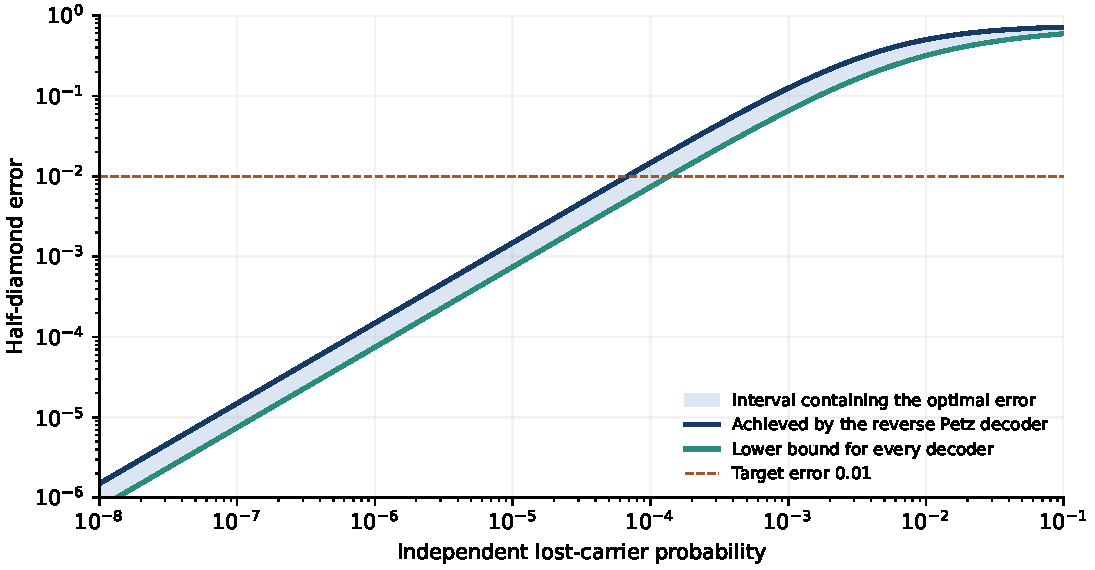
\includegraphics[width=\linewidth]{loss_bounds.pdf}
 \caption{Exact analytic infinite-count bounds at $\theta=0.1$. The shaded interval contains the optimal half-diamond error for independent flagged erasure. Neither boundary is asserted to be the exact optimum. The horizontal line is an error target of $0.01$. This plot evaluates formulas; it is not a simulation of a large quantum register.}
\end{figure}

\begin{center}
\begin{tabular}{rrrr}
\toprule
\shortstack{Loss\\probability} & \shortstack{Petz error\\$N=43\,462$} & \shortstack{Any-decoder bound\\$N=43\,462$} & \shortstack{Any-decoder bound\\$N\to\infty$}\\
\midrule
$0$ & $0.00999962$ & $0.00501659$ & $0$\\
$10^{-5}$ & $0.0113890$ & $0.00571628$ & $0.000747643$\\
$10^{-4}$ & $0.0236813$ & $0.0119356$ & $0.00737798$\\
$10^{-3}$ & $0.128466$ & $0.0672476$ & $0.0653091$\\
$10^{-2}$ & $0.501397$ & $0.318199$ & $0.318198$\\
\bottomrule
\end{tabular}
\end{center}
Thus losing one carrier in a thousand already prevents error $0.01$ at $\theta=0.1$, regardless of how long this independently erased stream is collected.

\subsection{Keeping only an untouched subset}
For a budget of at most $m$ untouched retained carriers, $a_N$ is maximized by retaining the first $m$. Exchange an adjacent erased--retained pair for retained--erased. The acquired coefficient increases by $b(1-d)q$, while the later residual coefficient is unchanged. Repeated exchanges give
\[
 a_N\le1-(1-b)^m.
\]
Consequently every decoder of any such subset needs
\begin{equation}
 m\ge\frac{\log\!\left[1/\{1-(1-4\epsilon/3)^2\}\right]}{-\log(1-b)}
\end{equation}
to achieve error $\epsilon<3/4$. Retaining the first $m$ and applying the inverse reader suffices when
\begin{equation}
 m\ge\frac{\log(3/(4\epsilon))}{-\log(1-b)}.
\end{equation}
The retained-carrier requirement in this class is therefore $\Theta(\theta^{-4}\log(1/\epsilon))$. Input-independent random selection does not improve the lower bound. The exchange argument optimizes the exact Gram/Petz coefficient; no claim is made that it exactly orders every subset by its optimal decoding error. In particular, this theorem does not cover coherent processing before discard.

\section{Constructions tested and their actual scopes}
Three constructors began separately with the channel formulation, an operational input/output specification, and an operator/MPO formulation. Separate prompts did not remove shared model training or make the attempts statistically independent. Mechanisms were exchanged only after concrete derivations were available.

The operational route recovered the inverse reader independently. It also ruled out a particular pure Bell dark-state absorber. A fresh tracial carrier can be purified by an inaccessible qubit; one source collision creates source--purifier correlation. Receiver operations cannot change that marginal, so they cannot restore an exact pure Bell state between source and receiver. This is a local obstruction, not a general memory theorem.

The folded inverse tensor is
\[
 V=cI-2is\Phi,\qquad V^\dagger V=c^2I+4s^2\Phi,
\]
with singular values $c$ and $\sqrt{1+3s^2}$. It is not an isometry. The earlier Astra note [A2] already proves that a particular two-qubit folded statistic is not causal and quantifies the postselection cost. A new constructive attempt completed this tensor to the valid instrument
\[
 K_k=\tfrac12V(P_k\otimes I),\qquad k=0,1,2,3,
 \qquad\sum_kK_k^\dagger K_k=I,
\]
where $P_k$ are the four Paulis. The outcome at the first step can be corrected using the initial receiver Bell pair, but discarding the processed carrier already loses information. With $x=\sin^2\theta$, the distinguishability of two opposite source inputs in the full source-plus-receiver state becomes
\[
 D_1=\frac{x+\sqrt{4(1-x)^4+4x-3x^2}}2<1\qquad(0<x<1).
\]
All corrected first branches agree, and the record is input-independent. No subsequent operation, even with the source granted, can increase that distinguishability. Thus this particular first-step discard forces final error at least $(1-D_1)/2=\theta^2/2-11\theta^4/12+O(\theta^6)$. Independent two-step checks also refute the proposed Pauli-frame closure. These statements exclude the specified mechanism, not every small receiver.

Other boundary calculations encountered here, including measured Schur compression, pair-sector pinching and purified-dummy block readers, were already treated in [A2]. They are not new results from this run. Pure-state tensor-network compression [4] also cannot be applied merely from a small mixed-state MPO bond; its operational premises must be met.

\section{Verification, provenance and limitations}
The crossing/intertwiner identities, interpolation, variance normalization and finite spectral bound were checked independently at prefixes $n=1,\ldots,4$ and five positive or negative values of $u$. All 20 cases passed; the largest relative identity/interpolation error was $3.4\times10^{-10}$, arising from degree-four interpolation cancellation. The crossing identities themselves had tighter residuals. These checks corroborate the analytic proof and do not replace it. The exact three-carrier coefficient matrix was also recomputed in rational symbolic arithmetic.

The retained-carrier recurrence was checked against dense channel matrices for every subset at $N=1,\ldots,5$ and $\theta\in\{0.1,0.4,0.9\}$: $186$ cases, with maximum Gram-entry discrepancy $4.44\times10^{-16}$. The proof above is independent of those floating-point checks. Large-count numerical rows evaluate the analytic recurrence only.

Additional finite singular-value calculations cover the full bath operator space through four carriers and the SU(2)-scalar operator sector through seven. The latter is a restricted invariant sector, not automatically the entire smallest-gap spectrum. Closure residuals are at floating-point scale. These computations do not establish large-$N$ behavior. The archive retains code and numerical receipts with that scope.

The quantitative crossing bound, sharpened witness coefficient, finite-memory floors and erasure extension were derived and combined during this investigation, using established recovery and R-matrix machinery. An exhaustive priority claim is not made. The erasure result concerns loss before receiver access and is not substituted for a general compression obstruction. The all-output operation, earlier general profile framework and prior restricted failures retain their attribution.

\Needspace{8\baselineskip}
\textbf{Resolution status.} No causal sublinear-memory decoder with the requested guarantee has been constructed. The general $\Omega_\theta(N/\log N)$ lower bound does not match the known $N$-qubit reader or settle the joint weak-angle limit. The fixed endpoint remains unresolved. What remains is either a physical causal compression with the full recovery and resource guarantees, or a sufficiently sharp general converse closing this gap. The present lower bound is not relabeled as a full resolution.

\section*{Sources}
\small
\begin{description}
\item[{[A1]}] Astra research knowledge, \emph{Tracial acquisition: partial-SWAP decoder}, return dated 5 November 2026. Repository \path{harjassand/astra-research-knowledge}. Pinned commit:\\ \texttt{fef3640a8b1dc5475674a006de417f652f3baf3c}. Governing source:\\ {\footnotesize\path{research/returns/2026-11-05-p2-tracial-acquisition/package/partial_swap_theory.txt}}.\\ Retrieved as research material, not represented as a peer-reviewed publication.
\item[{[A2]}] \emph{Causal memory for the homogeneous tracial partial-SWAP stream: Proved bounds, physically specified candidates, and the unresolved tradeoff}, 5 November 2026, 13-page Astra research note. Existing file \texttt{weak\_stream\_memory.pdf}. Identifier:\\ \texttt{libfile\_66a8b33dfd988191b76f181429691b90}. The prefix framework and restricted obstructions cited here are prior material.
\item[{[1]}] M. Ziman et al., \emph{Quantum homogenization}, Phys. Rev. A 65, 042105 (2002). \url{https://arxiv.org/abs/quant-ph/0110164}.
\item[{[2]}] J. M. Renes, \emph{Better bounds on optimal measurement and entanglement recovery, with applications to uncertainty and monogamy relations}, Phys. Rev. A 96, 042328 (2017). \url{https://arxiv.org/abs/1707.01114}.
\item[{[3]}] C. C. Aw, L. H. Zaw, M. Balanz\'o-Juand\'o and V. Scarani, \emph{Role of dilations in reversing physical processes: Tabletop reversibility and generalized thermal operations}, PRX Quantum 5, 010332 (2024). \url{https://arxiv.org/abs/2308.13909}.
\item[{[4]}] G. Bai, Y. Yang and G. Chiribella, \emph{Quantum compression of tensor network states}, New J. Phys. 22, 043015 (2020). \url{https://doi.org/10.1088/1367-2630/ab7a34}.
\item[{[5]}] P. W. Claeys, J. Herzog-Arbeitman and A. Lamacraft, \emph{Correlations and commuting transfer matrices in integrable unitary circuits}, SciPost Phys. 12, 007 (2022). \url{https://arxiv.org/abs/2106.00640}.
\end{description}
\end{document}
